\chapter{Linear elasticity equation -- 2D -- Loaded elastic beam}

\modinfo{Directory}{ElasticBeam2D}
\modinfo{Solvers}{\Idx{StressSolve}}
\modinfo{Tools}{\Idx{ElmerGUI}}
\modinfo{Dimensions}{2D, Steady-state}
\modinfo{Author}{Peter R{\aa}back}


\subsection*{Case definition}

A homogenous, elastic beam ($\Omega$) is rigidly supported on one 
end (boundary $\Gamma_4$). On boundary $\Gamma_3$ the beam is subjected 
to a load $q(x)$, which grows linearly from zero to $q_0$ 
(see figure~\ref{fg:beam}). The length of the beam is 1~m and the thickness 0.1~m.
Material properties of the beam are those of iron (in the database) Poisson 
ratio 0.29 and Young's modulus $193\cdot 10^9$N/m$^2$. Problem is to solve the 
displacement of the beam.  

\begin{figure}[h]
\centering
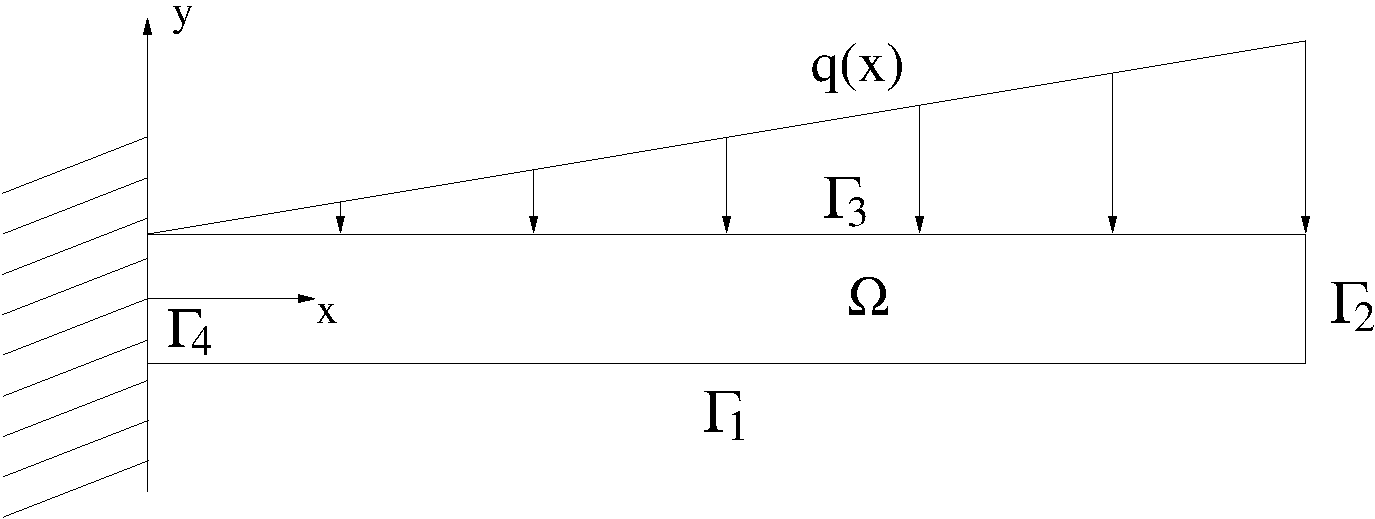
\includegraphics[width=100mm]{Beam}
\caption{Beam and loading.}\label{fg:beam}
\end{figure}

Problem is solved according to linear elasticity theory. Mathematically 
the problem to be solved is
\begin{equation}
\left \{
\begin{array}{rcll}
-div \sigma & = & 0 & \mbox{ in } \Omega \\
\sigma & = & \lambda tr [\varepsilon(u)]I + 2 \mu \varepsilon(u) &
\mbox{ in } \Omega \\
u & = & 0 & \mbox{ on } \Gamma_4 \\
\sigma n & = & 0 & \mbox{ on } \Gamma_1 \cup \Gamma_2 \\
\sigma n & = & -q & \mbox{ on } \Gamma_3 \\
\end{array}
\right .
\end{equation}
where $\lambda$ and $\mu$ are the Lam\'{e} constants (which can be expressed 
in terms of the Poisson ratio and Young's modulus), $\varepsilon$ is the 
linearised strain tensor, $u$ is the displacement vector, $q$ is the given
surface traction and $n$ is the outward unit normal to the boundary.



\subsection*{Solution procedure}

The mesh is given in ElmerGrid format in file \texttt{beam.grd}, load this file.
\ttbegin
File 
  Open -> beam.grd
\ttend
You should obtain your mesh, \texttt{Model, Summary...} and may check that
it consists of 1000 biquadratic elements.
\begin{figure}[h!]
\begin{center}
  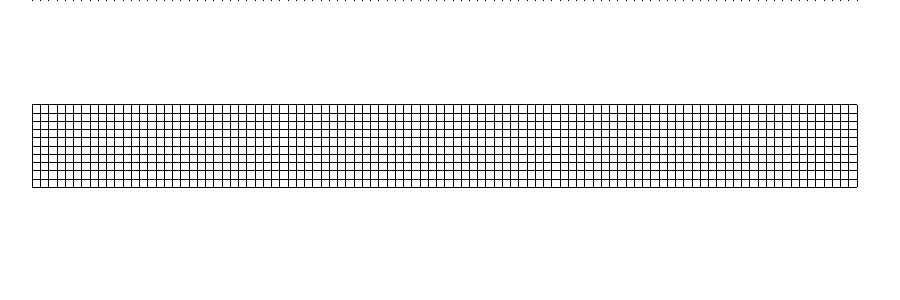
\includegraphics[width=0.8\textwidth,viewport=0 30 900 270,clip]{beammesh}
  \caption{The mesh used in the computations}
  \label{fig:elast_mesh}
\end{center}
\end{figure}

After we have the mesh we start to go through the Model menu from the top to bottom. 
In the Setup we choose things related to the whole simulation such as file names, 
time stepping, constants etc.
The simulation is carried in steady-state in 2-dimensional Cartesian coordinates. 
\ttbegin
Model
  Setup 
    Simulation Type = Steady state
    Steady state max. iter = 1
\ttend

In the Equation section we choose the relevant equations which in this case only includes 
the \texttt{Linear elasticity} equation which solves the problem according to 
linear elastic theory.
In this case we assume that the beam is thin in the $z$-direction and hence assume plane stresses.
When defining Equations and Materials it is possible to assign to the bodies immediately, or to use mouse
selection to assign them later. In this case we have just one body and therefore its easier to assign 
the Equation and Material to it directly.
For the linear system solvers we are happy to use the defaults. One may however, try out different
preconditioners (ILU1,\ldots) or direct Umfpack solver, for example.
\ttbegin
Model
  Equation
    Name = Elasticity
    Apply to Bodies = 1
    Linear elasticity
      Active = on
      Plane Stress = True
    Add 
    OK
\ttend        
The Material section includes all the material parameters.
They are divided to generic parameters which are direct properties of the material
without making any assumptions on the physical model, such as the mass. Other properties assume
a physical law, such as conductivities and viscosity. 

Here we choose the generic iron from the material library.
You may click through the material parameters of the various solvers to ensure that
the properties are indeed as they should be. Any consistent set of units may be used in Elmer.
The natural choice is of course to perform the computations in SI units. 

\ttbegin
Model
  Material
    Material library    
      Iron (generic)
    Apply to Bodies = 1 
    Add
    OK
\ttend

There are no body forces and convergence should be easily obtained with the default 
initial condition i.e. zero for all fields.

The first boundary condition fixes the beam rigidly at the wall.
The second boundary condition may seem confusing. Basically it represents the form 
using a linear interpolation between two points. At $x=0$ the force $f_y = 0$ and 
at $x=1$ the force $f_y=-1.0e7$, respectively. The semicolon is an alternative separator
to line break. To fill in the second boundary condition press \texttt{Enter} in the 
\texttt{Force 2} checkbox.
\ttbegin
Model
  BoundaryCondition
    Name = Wall
    Linear elasticity
      Displacement 1 = 0.0
      Displacement 2 = 0.0
    Add
    New

    Name = Top
    Linear elasticity 
      Force 2 = Variable Coordinate 1; Real; 0 0; 1 -1.0e7; End
    Add 
\ttend   

The conditions may also be assigned to boundaries in the Boundary condition menu, or 
by clicking with the mouse. Here we use the latter approach as that spares us of the 
need to know the indexes of each boundary.
\ttbegin
Model
  Set boundary properties
    Choose left-hand-side -> set boundary condition Wall
    Choose top -> set boundary condition Top
\ttend

For the execution 
ElmerSolver needs the mesh files and the command file. We have now basically defined
all the information for ElmerGUI to write the command file. After writing it we may also visually 
inspect the command file.
\ttbegin
Sif 
  Generate
  Edit -> look how your command file came out  
\ttend

Before we can execute the solver we should save the files in a directory. The project includes
all the files needed to restart the case.
\ttbegin
File 
  Save Project
\ttend

After we have successfully saved the files we may start the solver
\ttbegin
Run
  Start solver
\ttend
A convergence view automatically pops up showing relative changes of each iteration.
Two iterations are performed, the second one only to ensure convergence at the nonlinear level.
The norm of the finished computation should be around 0.01808.

When there are some results to view we may start the postprocessor also
\ttbegin
Run
  Start ParaView
\ttend


\subsection*{Results}

As a result the absolute value of maximum displacement is given. The 
displacements calculated with different load values $q_0$ are tabulated in 
table~\ref{tb:struct3a}. Note that the absolute value of the
displacement varies linearly with respect to the load since the model
is linear.

\begin{figure}[h!]
\begin{center}
  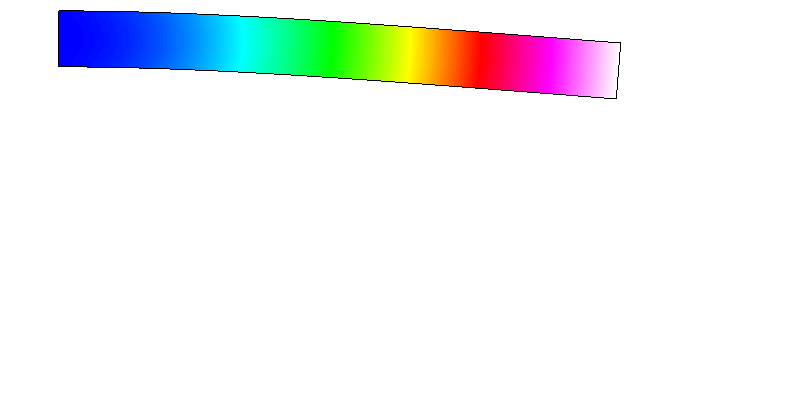
\includegraphics[width=0.4\textwidth,angle=0]{beam1.png}
  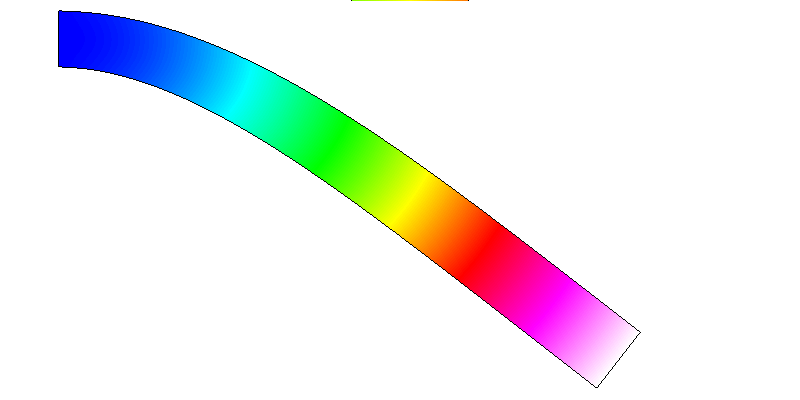
\includegraphics[width=0.4\textwidth,angle=0]{beam2.png}
  \caption{The displacement of an elastic beam with two different loads
using a linear model}
  \label{fig:elast_beam1}
\end{center}
\end{figure}

\begin{table}[h]
\caption{Displacements with different load values}
\label{tb:struct3a}
\begin{center}
\begin{tabular}{ll} \hline
$q_0$ [N/m$^2$] & $\max |u|$ [m] \\ \hline
-1.0$e7$ & 0.05755 \\
-1.0$e8$ & 0.5755 \\
-1.0$e9$ & 5.755 \\ \hline
\end{tabular}
\end{center}
\end{table}

If you look at the results you can see that the displacement values
become relatively large. The linear theory is valid only to small 
displacements. From Fig~\ref{fig:elast_beam1} you can also notice that the
beam does not maintain its original form. This means that the linear 
elasticity theory can not take into consideration all the necessary 
phenomena that are related to the problem, any more. To be able to 
solve the problem we must use general elasticity theory.


\subsection*{Extra task: transient loading}

If you have time you may try to solve the case using transient loading. 
You may try with the following settings.
\ttbegin
Model
  Setup 
    Simulation Type = Transient
    Time Stepping Method = bdf
    BDF Order = 2
    Time Step Intervals = 200
    Time Step Sizes = 1.0e-4
\ttend
Having a too large time step will not accurately describe the transient behaviour while having a too 
small time step consumes unnecessary resources. There is only numerical damping in the system and 
hence it will oscillate for some time.
%To visualize the oscillations set in the \texttt{Time Step Control} 
%in the \texttt{Do after frame} box the following command
%\ttbegin
%  math nodes=n0+Displacement(0:2,time($t))
%\ttend
%It will add the right timestep of the displacement field to the initial coordinate values.

 

\vfill
\mbox{}
